%% LyX 2.0.7.1 created this file.  For more info, see http://www.lyx.org/.
%% Do not edit unless you really know what you are doing.
\documentclass[english]{beamer}
\usepackage[T1]{fontenc}
\usepackage[latin9]{inputenc}
\usepackage{listings}
\setcounter{secnumdepth}{3}
\setcounter{tocdepth}{3}
\setlength{\parindent}{0bp}
\usepackage{amssymb}
\usepackage{graphicx}
\usepackage{esint}

\makeatletter
%%%%%%%%%%%%%%%%%%%%%%%%%%%%%% Textclass specific LaTeX commands.
 % this default might be overridden by plain title style
 \newcommand\makebeamertitle{\frame{\maketitle}}%
 \AtBeginDocument{
   \let\origtableofcontents=\tableofcontents
   \def\tableofcontents{\@ifnextchar[{\origtableofcontents}{\gobbletableofcontents}}
   \def\gobbletableofcontents#1{\origtableofcontents}
 }
 \long\def\lyxframe#1{\@lyxframe#1\@lyxframestop}%
 \def\@lyxframe{\@ifnextchar<{\@@lyxframe}{\@@lyxframe<*>}}%
 \def\@@lyxframe<#1>{\@ifnextchar[{\@@@lyxframe<#1>}{\@@@lyxframe<#1>[]}}
 \def\@@@lyxframe<#1>[{\@ifnextchar<{\@@@@@lyxframe<#1>[}{\@@@@lyxframe<#1>[<*>][}}
 \def\@@@@@lyxframe<#1>[#2]{\@ifnextchar[{\@@@@lyxframe<#1>[#2]}{\@@@@lyxframe<#1>[#2][]}}
 \long\def\@@@@lyxframe<#1>[#2][#3]#4\@lyxframestop#5\lyxframeend{%
   \frame<#1>[#2][#3]{\frametitle{#4}#5}}
 \def\lyxframeend{} % In case there is a superfluous frame end

%%%%%%%%%%%%%%%%%%%%%%%%%%%%%% User specified LaTeX commands.
\usetheme[secheader]{Madrid}

\makeatletter
\setbeamertemplate{footline}
{
  \leavevmode%
  \hbox{%
  \begin{beamercolorbox}[wd=.333333\paperwidth,ht=2.25ex,dp=1ex,center]{author in head/foot}%
    \usebeamerfont{author in head/foot}{Methods and Computing}
  \end{beamercolorbox}%
  \begin{beamercolorbox}[wd=.333333\paperwidth,ht=2.25ex,dp=1ex,center]{title in head/foot}%
    \usebeamerfont{title in head/foot}{Harvard Univeristy}
  \end{beamercolorbox}%
  \begin{beamercolorbox}[wd=.333333\paperwidth,ht=2.25ex,dp=1ex,right]{date in head/foot}%
    \usebeamerfont{date in head/foot}{Department of Biostatistics}
    \insertframenumber{} / \inserttotalframenumber\hspace*{2ex} 
  \end{beamercolorbox}}%
  \vskip0pt%
}
\makeatother

\makeatother

%% Update the formatting of \alert{}
\setbeamerfont{alerted text}{series=\bfseries}
\setbeamercolor{alerted text}{fg=black}

\usepackage{babel}
\begin{document}


\title{Biostatistics Preparatory Course:\\
Methods and Computing}


\author{Lecture 3}

\date{Probability Distributions}

\makebeamertitle

\lyxframeend{}\lyxframe{Yay Rmarkdown!}

\begin{itemize}
\item Install LaTeX on your computer
\item Download the '2018\_Lecture3\_Exercises.Rmd' from the course website
\item Open file in R 
\item Choose 'Knit to pdf' and cross your fingers
\end{itemize}
\lyxframeend{}


\lyxframeend{}\lyxframe{Probability Distributions}
\begin{itemize}
\item In statistics, we try to draw conclusions about a larger population
from a sample of observations
\item We use mathematical models to capture probabilistic behavior of a
population
\item This behavior is modeled using probability distributions
\end{itemize}

\lyxframeend{}

 \lyxframeend{}\lyxframe{Density/Distribution Functions}
\begin{definition}[Cumulative Distribution Function]
	\centering
	$F_{X}\left(x\right)=P\left(X\le x\right)$
	$\forall x\in\mathbb{R}$
\end{definition}
\begin{itemize}
	\item A CDF is associated with every RV $X$
	\item A RV is continuous if $F_{X}\left(x\right)$ is continuous in
	$x$, and discrete if $F_{X}\left(x\right)$ is a step function in $x$
	\begin{itemize}
		\item A discrete RV takes on a finite/countable number of values,
		e.g. subset of natural numbers
		\item A continuous RV takes on value from some uncountable subset of
		the reals
	\end{itemize}
\end{itemize}

\lyxframeend{}



 \lyxframeend{}\lyxframe{Density/Distribution Functions cont.}
 \begin{definition}[Probability Mass Function]
 For a discrete RV, the \alert{probability mass function (PMF)} is:\\
 \[
 f_{X}\left(x\right)=P\left(X=x\right) \forall x\in\mathbb{R}
 \]
 \end{definition}
\pause
 \begin{definition}[Probability Density Function]
   For a continuous RV, the \alert{probability density function (PDF)}
   is:
 \[
 f_{X}\left(x\right)= \frac{\partial}{\partial t} F(t) \big
 |_{t=x}
 \]
 So $F_{X}(x) = \int_{-\infty}^{x}f_{X}\left(t\right)dt \forall
 x\in\mathbb{R}$.
 \end{definition}

 Note that $f_{X}\ge0$ for $\forall x$, and thus $F_{X}$ is an
 increasing function

 \lyxframeend{}


 \lyxframeend{}\lyxframe{Expectation and Variance}
 \begin{definition}[Expectation]
 A measure of central tendancy (a weighted average of the values of
 $X$)
 \[
   E\left[X\right]=\sum_{x \in S} x \ P(X=x)  \text{ for discrete RV taking
   values from $S$}
 \]
 \[
 E\left[X\right]=\int_{-\infty}^{\infty}x \ f_X(x)dx \text{ for continuous RV}
 \]
 \end{definition}
\pause
 \begin{definition}[Variance]
 A measure of the spread of a distribution
 \begin{center}
   $Var(X)=\sum_{x\in S}\left(x-E\left[X\right]\right)^{2} \ P(X=x) $
    for discrete RV \\
    
 $Var(X)=\int_{-\infty}^{\infty}\left(x-E\left[X\right]\right)^{2} f_X(x)dx$
  for continuous RV
 \end{center}
 \end{definition}
\lyxframeend{}


 \lyxframeend{}\lyxframe{Example of Continuous Distribution (Normal)}
 \begin{itemize}
 \item The normal distribution is a very important distribution because:

 \begin{itemize}
 \item A lot of things look normal
 \item Analytically tractable
 \item Central limit theorem
 \end{itemize}
 \item $f_{X}\left(x\right)=\frac{1}{\sqrt{2\pi} \sigma}exp\left(-\frac{\left(x-\mu\right)^{2}}{2\sigma^{2}}\right)$
 for $\forall x\in\mathbb{R}$
 \item Characterized by mean, $\mu$, and variance, $\sigma^{2}$
 \end{itemize}
 \begin{center}
 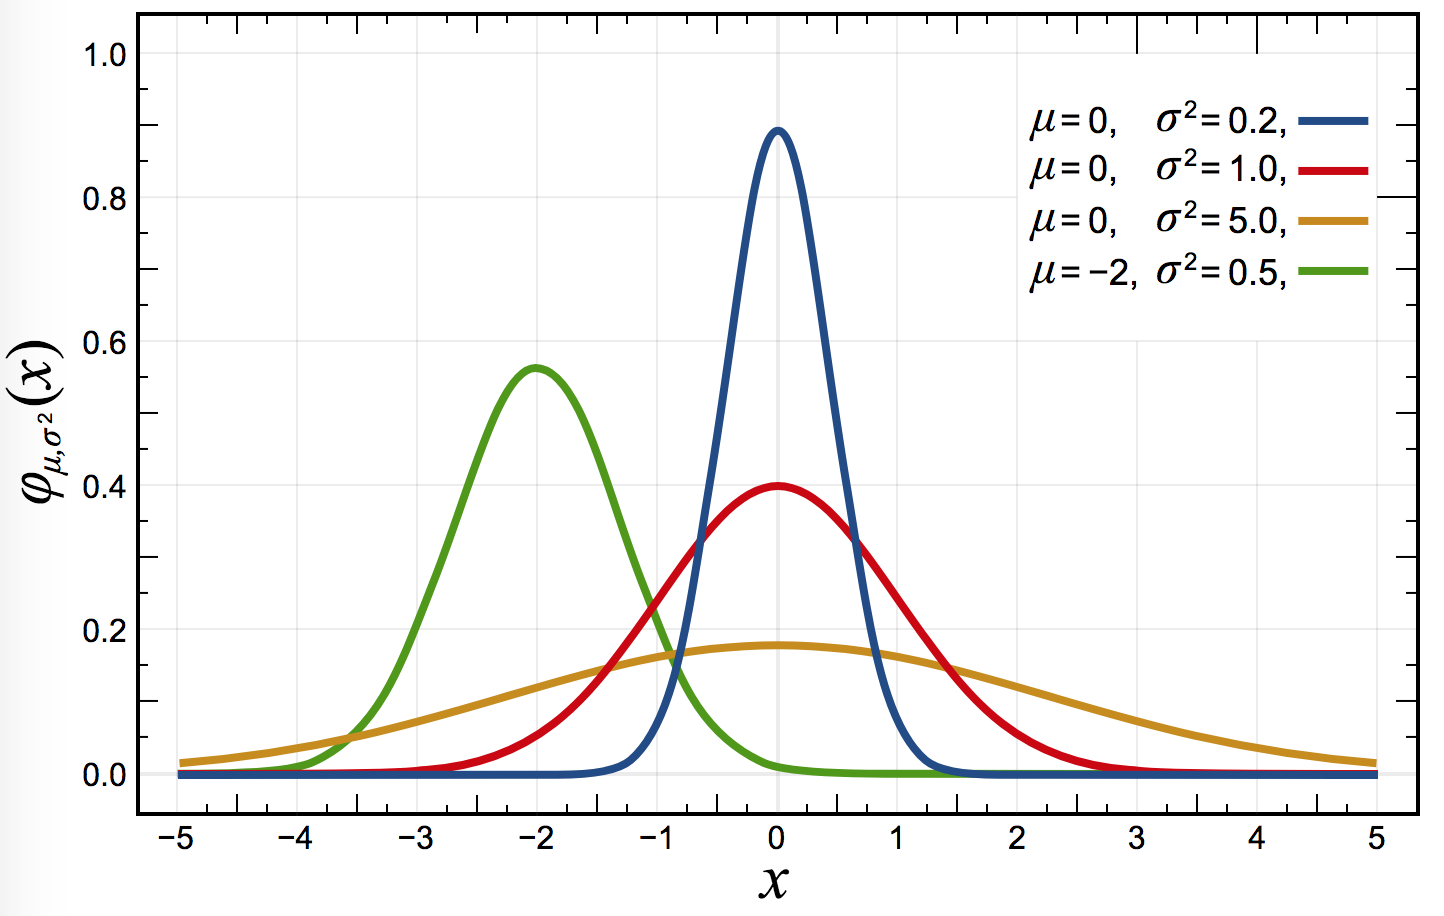
\includegraphics[width=0.5\textwidth]{dnorm}
 \par\end{center}


 \lyxframeend{}

 \begin{frame}[fragile]{How to Generate Samples from Normal Distribution}
 
 	
 	\noindent The following commands are for a normal random variable with mean $\mu$ and variance $\sigma^2$, that is, $X \sim N(\mu, \sigma^2)$, 
 	
 	\begin{itemize}
 \item To calculate the probability density function at a value $x$, i.e. $f_X(x)$ 
 
 \begin{lstlisting}[basicstyle={\footnotesize\ttfamily},language=R,showstringspaces=false]
 dnorm(x,mu,sigma)
 \end{lstlisting}
 
 \item To calculate the cumulative distribution function at a value $x$, i.e. $P(X \leq x)$ 
 
 \begin{lstlisting}[basicstyle={\footnotesize\ttfamily},language=R,showstringspaces=false]
  pnorm(x,mu,sigma) 
 \end{lstlisting}

 \item To generate a size $m$ sample from the normal distribution, i.e. $X_1, ..., X_m$ where $X_i \sim N(\mu, \sigma^2)$. 
 
 \noindent 
 \begin{lstlisting}[basicstyle={\footnotesize\ttfamily},language=R,showstringspaces=false]
 rnorm(m,mu,sigma)
 \end{lstlisting}


 \item Note that the third argument is the \textbf{square root of the variance}, this
 is because the R function for normal distribution asks for the standard
 deviation, which is defined as the square root of the variance
 \end{itemize}
 \end{frame}

\begin{frame}[fragile]{Normal Distribution Exercises}
\end{frame}

\begin{frame}[fragile]{In general: Probability Distributions in R}
\begin{itemize}
	\item Many probability distributions are defined in R 
	\item All common distributions (and most others) have four functions
	associated with them:
	\begin{itemize}
		\item {\bf Density}: the probability mass function for discrete or
		the probability density function for continuous random
		variables. Prefixed by \verb+d+ (eg., \verb+dnorm+).
		\item {\bf Distribution function}: the cumulative distribution
		function, $P(X \leq x)$. Prefixed by \verb+p+ (eg., \verb+pnorm+).
		\item {\bf Quantile function}: The inverse cdf. Prefixed by \verb+q+
		(eg., \verb+qnorm+).
		\item {\bf Random generation}: Generate $n$ random values from the
		distribution. Prefixed by \verb+r+ (eg., \verb+rnorm+).
	\end{itemize}
	\item Using \verb+?+ with any of the four functions brings the help
	for all of them (eg., \verb+?rnorm+).
\end{itemize}
\end{frame}

 \lyxframeend{}\lyxframe{Example of Discrete Distribution (Binomial)}
 \begin{itemize}
 \item $\mbox{Bernoulli}\left(p\right)$ RV, is 1 with probability $p$ and
 0 with probability $1-p$
 \item $\mbox{Binomial}\left(n,p\right)$ RV, sum of $n$ independent $\mbox{Bernoulli}\left(p\right)$
 RV

 \begin{itemize}
 \item Fixed number, $n$, of Bernoulli trials
 \item Each trial has the same probability of success
 \end{itemize}
 \item $f_{X}\left(k\right)=P\left(X=k\right)=\left(\begin{array}{c}
 n\\
 k
 \end{array}\right)p^{k}\left(1-p\right)^{n-k}$ for $k=0\ldots n$
 \item Characterized by $p$ and $n$
 \end{itemize}

 \begin{center}
	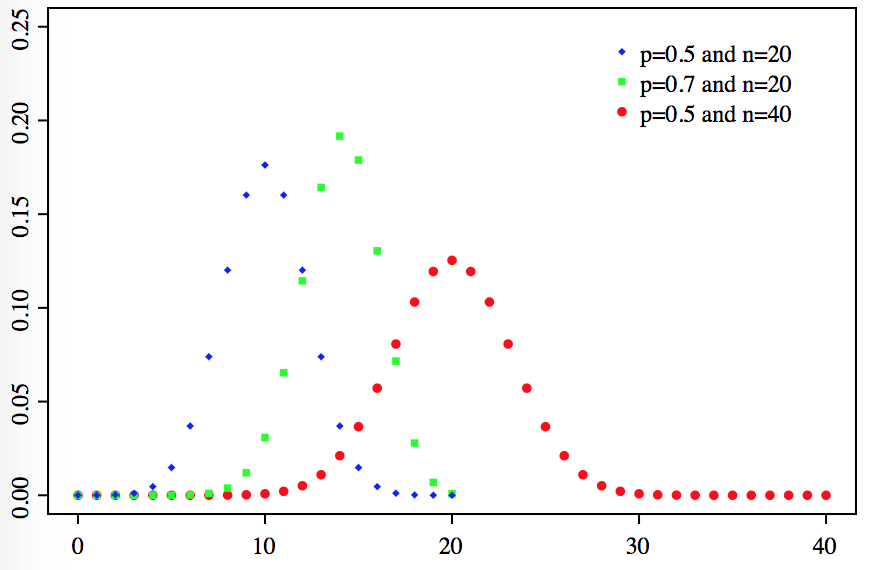
\includegraphics[width=0.5\textwidth]{binom}
	\par\end{center}

 \lyxframeend{}
 
  \lyxframeend{}\lyxframe{Example of Discrete Distribution (Poisson)}
 \begin{itemize}
 	\item $\mbox{Poisson}\left(\lambda\right)$ RV has an event rate $\lambda > 0$
 	\item $f_{X}\left(k\right)=P\left(X=k\right)= e^{-\lambda} \frac{\lambda^k}{k!}$ for $k=0, 1, 2,\ldots$
 	\begin{itemize}
 		\item $k$ can be thought of as the number of events that occur in a given time period or space
 		\item $\lambda$ can also be though of as the mean number of events that occur in a given time period or space as $E[X] = \lambda$
 	\end{itemize}
 	\item Characterized by $\lambda$
 \end{itemize}
 
 \begin{center}
 	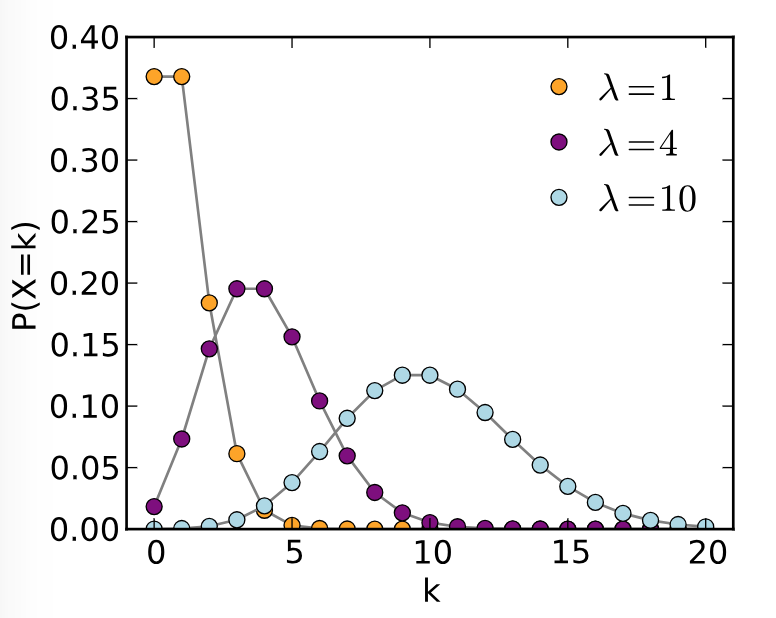
\includegraphics[width=0.5\textwidth]{poisson}
 	\par\end{center}
 
 \lyxframeend{}


\begin{frame}[fragile]{Some Probability Distributions in R: The Most Common}
\begin{center}
\begin{tabular}{c|c|c}
  \textbf{Distribution} &  \textbf{R Abbrev} & \textbf{Description} \\
  \hline
  Normal & \verb+norm+ & everyone's favorite bell curve \\
  \hline
  $t$ & \verb+rt+ & \begin{minipage}[c]{6cm} standard normal distribution with wider tails \end{minipage} \\
  \hline
  Uniform &  \verb+unif+ & \begin{minipage}[c]{6cm} equal probability on the chosen interval \end{minipage}\\
  \hline \hline
  Binomial &
  \verb+binom+ & \begin{minipage}[c]{6cm}probability for a given number of successes in a fixed number of experiments \end{minipage}\\
  \hline
  Poisson & \verb+pois+ & \begin{minipage}[c]{6cm}probability of a given number of events occurring in a fixed interval of time or space \end{minipage} \\
  \hline
  Geometric & \verb+geom+ & \begin{minipage}[c]{6cm}probability that it takes a given number of failures until one success \end{minipage} \\
  \hline
\end{tabular}
\end{center}
\end{frame}

%\begin{frame}[fragile]{Probability Distributions R}
%\includegraphics[width=4in]{figure1.jpg}
%\end{frame}

\begin{frame}[fragile]{Some Probability Distributions in R: Other
    Useful Ones}
Continuous 
\begin{itemize}
\item Beta (\verb+?rbeta+)
\item Chi-sq (\verb+?rchisq+)
\item Exponential (\verb+?rexp+)
\item F (\verb+?rf+)
\item Logistic (\verb+?rlogis+)
\item Lognormal (\verb+?rlnorm+)
\end{itemize}

Discrete
\begin{itemize}
	\item Geometric (\verb+?rgeom+)
	\item Negative Binomial (\verb+?rnbinom+)
	\item Multinomial (\verb+?rmultinom+)
\end{itemize}

\end{frame}

\begin{frame}[fragile]{Empirical vs. Theoretical CDF}

In statistics, an empirical distribution function is the distribution function associated with the empirical measure of a \textbf{sample}. \\

We can denote the theoretical CDF as (this is what dnorm gives you!): 
$$F_X(k) = Pr(X \leq k)$$ 
and the empirical as: 
$$\hat{F}_n(k) = \frac{\textrm{number of elements in the sample} \leq k}{n} = \frac{1}{n} \sum_{i=1}^n I_{X_i \leq k} $$
where $X_1, ..., X_n$ make up some random sample from the underlying distribution.

\end{frame}


\begin{frame}[fragile]{Poisson Distribution Exercises}
\end{frame}




\begin{frame}[fragile]{Group Exercises}
\end{frame}

\end{document}